\documentclass[onecolumn, oneside, a4paper, 11pt]{memoir}

\usepackage[utf8]{inputenc}
\usepackage[T1]{fontenc}

% Paths
\newcommand{\figs}{../figs}
\newcommand{\data}{../data}

% Fonts
\usepackage{newpxtext,newpxmath}
\renewcommand*\sfdefault{cmss}

% References
\usepackage{hyperref}

% Units
\usepackage[detect-weight=true, binary-units=true]{siunitx}
\DeclareSIUnit\flop{Flops}

% Math
\let\openbox\undefined
\usepackage{amsthm}
\usepackage{amsmath}
\usepackage{amssymb}
\usepackage{bm}

\theoremstyle{remark}
\newtheorem{ex}{Question}
\newtheorem*{sol}{Solution}

% Graphics
\usepackage{graphicx}
\usepackage{caption}
\usepackage{subcaption}
\graphicspath{{../figs/}}

% Tikz
\usepackage{tikz}
\usetikzlibrary{positioning,shapes,arrows,calc,intersections}
\usepackage{pgfplots}
\usepgfplotslibrary{dateplot}
\pgfplotsset{compat=1.8}

% Colors
\definecolor{darkblue}{HTML}{00688B}
\definecolor{darkgreen}{HTML}{6E8B3D}
\definecolor{cadet}{HTML}{DAE1FF}
\definecolor{salmon}{HTML}{FFB08A}

% Listings
\usepackage{textcomp}
\usepackage{listings}
\lstset{
  keywordstyle=\bfseries\color{orange},
  stringstyle=\color{darkblue!80},
  commentstyle=\color{darkblue!80},
  showstringspaces=false,
  basicstyle=\ttfamily,
  upquote=true,
}
\lstdefinestyle{fortran}{
  language=Fortran,
  morekeywords={for},
  deletekeywords={status},
}
\lstdefinestyle{c}{
  language=C,
  morekeywords={include},
}
\lstdefinestyle{shell}{
  language=bash,
}


\newcommand{\xx}{{\boldsymbol x}}
\newcommand{\mG}{{\mathrm G}}
\newcommand{\mQ}{{\mathrm Q}}
\newcommand{\mS}{{\mathrm S}}
\newcommand{\mT}{{\mathrm T}}
\newcommand{\mU}{{\mathrm U}}
\newcommand{\mEVa}{{\Lambda}}

\begin{document}

\pagestyle{empty}

\begin{center}
  {\Huge \bfseries \scshape
    Introduction to \\[0.2\baselineskip] Supercomputing} \\[2\baselineskip]
  {\Large TMA4280 $\cdot$ Project II} \\[2\baselineskip]
\end{center}

\textbf{This project is mandatory, counts for 30\% of the final grade and can be done in pairs or alone.}

\section*{Instructions}

The deadline is set on the \textbf{19th of April 2017}.


\medskip
The deliverable consists of:
\begin{enumerate}
\item a report describing your solution, handed out by email in PDF format,
\item the source code developed to perform the computations stored in the same GIT repository as Project I,
\item a 5 minute demonstration of the code on the 19th of April highlighting the main results obtained.
\end{enumerate}

\medskip
Practical requirements regarding the code:
\begin{enumerate}
\item it should be hosted on \href{https://github.com/}{Github},
\item it should be structured in different subdirectories addressing the different questions and results gathered in text files,
\item it must be written in C/C++ (without use of \texttt{std::vector}) or FORTRAN,
\item it must use double precision,
\item it must compile and run using Makefile targets,
\item results presented in the report have to be reproducible.
\end{enumerate}

As soon as you have decided whether you want to work in pairs or alone:
\begin{itemize}
\item create a Github repository (one per pair) named \texttt{TMA4280LABS} if it is not the case already,
\item send your name(s) and the link to the repository by email.
\end{itemize}

\setsecnumdepth{none}
\maxsecnumdepth{none}

\section{Problem description}

This project deals with the parallelization of the Fast-Diagonalization method introduced in Chapter 9 of the \href{http://thebb.github.io/TMA4280/notes.pdf}{Lecture Notes}.
Consider the solution $u$ to the two-dimensional Poisson problem with homogeneous Dirichlet boundary conditions,
\begin{align}
  \label{eq:poisson}  -\Delta u(\xx) &= f(\xx) & \xx \in \Omega = (0,1) \times (0,1), \\
  \label{bc:poisson}  u(\xx) &= 0 & \xx \in \partial\Omega.
\end{align}
with $f$ a given right-hand side.

\medskip
Problem \eqref{eq:poisson}--\eqref{bc:poisson} is approximated by a finite difference method on a regular grid with $(n+1)$ points in each spatial direction, with the grid size $h=1/n$,

\begin{center}
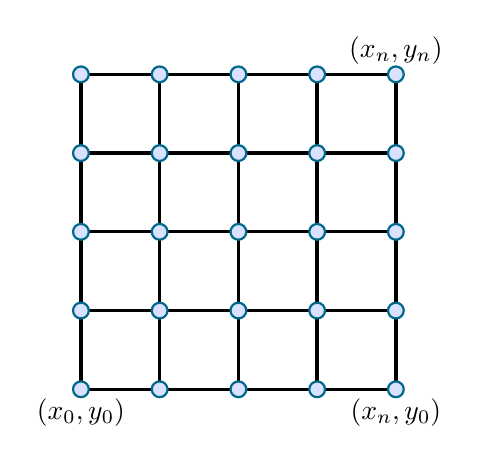
\begin{tikzpicture}
  \foreach \i in {0,...,4} {
    \draw[very thick] (\i,0) -- (\i,4);
    \draw[very thick] (0,\i) -- (4,\i);
  }
  \foreach \i in {0,...,4} {
    \foreach \j in {0,...,4} {
      \draw[thick, darkblue, fill=cadet] (\i,\j) circle (0.1);
    }
  }
  \node[anchor=north] at (0,0) {$(x_0, y_0)$};
  \node[anchor=north] at (4,0) {$(x_n, y_0)$};
  \node[anchor=south] at (4,4) {$(x_n, y_n)$};
\end{tikzpicture}
\end{center}
and the Laplace operator is discretized by the standard 5-point stencil,
\begin{center}
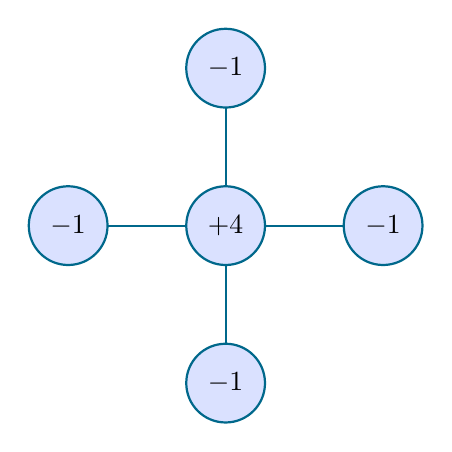
\begin{tikzpicture}[
  every node/.style={
    shape=circle,
    thick,
    fill=cadet,
    draw=darkblue,
    minimum size=1cm,
  }]
  \draw[thick, darkblue] (-2,0) -- (2,0);
  \draw[thick, darkblue] (0,-2) -- (0,2);
  \node at (-2,0) {$-1$};
  \node at (2,0) {$-1$};
  \node at (0,-2) {$-1$};
  \node at (0,2) {$-1$};
  \node at (0,0) {$+4$};
\end{tikzpicture}
\end{center}
for which the discrete equations read:
\begin{equation}
- \frac{u_{i+1,j} - 2 u_{i,j} + u_{i-1,j}}{h^2} - \frac{u_{i,j+1} - 2 u_{i,j} + u_{i,j-1}}{h^2} = f_{i,j}
\end{equation}
where $v_{i,j} = v(x_i,y_j)$ denotes the degree of freedom located at node $(i,j)$.
The solution vector can be represented in a matrix form
\[
\mU =
\begin{bmatrix}
u_{1,1}   & \cdots   &  \cdots    & \cdots   & u_{1, n-1}   \\
\vdots    & \ddots   &  \hfill    & \hfill   & \vdots       \\
\vdots    & \hfill   &  u_{i,j}   & \hfill   & \vdots       \\
\vdots    & \hfill   &  \hfill    & \ddots   & \vdots       \\
u_{n-1,1} & \cdots   &  \cdots    & \cdots   & u_{n-1, n-1} \\
\end{bmatrix}
\]
and the one-dimensional Laplace operator reads
\[
\mT = 
\begin{bmatrix}
2         & -1     &  0    & \cdots     & 0  \\
-1        &  2     &  -1    & \hfill    & \vdots       \\
0         & \ddots &  \ddots    & \ddots &  0       \\
\vdots    & \hfill &  -1     &  2   & -1       \\
0         & \cdots   &  0    & -1   & 2 \\
\end{bmatrix}
\]
so that in matrix form the two-dimensional problem may be written:
\begin{equation}
\mT\mU + \mU\mT = \mG
\end{equation}
with $\mG$ the matrix representing the right-hand side.

\medskip
Let us recall that such diagonalization methods consists of two \textit{matrix--vector} multiplications and one \textit{vector} operation in one dimension of space, while it requires four \textit{matrix--matrix} operations and one \textit{matrix} operation in two dimensions of space:
\begin{enumerate}
\item $\tilde\mG = \mQ^T\mG\mQ$
\item $\mEVa\tilde\mU + \tilde\mU\mEVa= \tilde\mG$
\item $\mU = \mQ\tilde\mU\mQ^T$
\end{enumerate}
with $\lambda$ the matrix of eigenvalues, and $\mQ$ the matrix of (orthonormal) eigenvectors, where $\mQ^{-1} = \mQ^T$.
The algorithm takes advantage of the fact that eigenvalues and eigenvectors can be computed explicitly.
To optimize further the algorithm the Discrete Sine Transform (DST) can applied to compute $\tilde\mU$ and $\tilde\mG$, with the substitution described in Chapter 9:
\[
\mQ = \sqrt{\frac{2}{n}} \mS^{-1}\qquad
\]
The problem was shown to be computable in $\mathcal{O}(n^2\log n)$ floating-point operations.

\bigskip
\begin{ex}
  Write a program to solve the Poisson problem with $P$ processes using the
  algorithm described. You can choose $f \equiv 1$ for the initial
  development.

  Use the provided routines to compute the DST and its inverse based on the FFT.
  See Appendix A for details on compiling, linking and running the serial
  version of the Poisson solver. Use the MPI communication library to develop
  your program for a distributed memory parallel computer, and OpenMP to use $t$
  threads on each MPI process. See Appendix C for comments on the transpose
  operation.
\end{ex}

\bigskip
\begin{ex}
  Run your parallel program on \emph{Lille}. Obtain detailed timing results for
  different combinations of $n=2^k$ and $P, t$. In particular, demonstrate that
  your program functions correctly for selected values of $P$ in the range
  $1 \leq P \leq 36$. Follow the procedure described in Appendix B.

  \textbf{Note:} Having a program that runs quickly is useless unless the answer
  is correct.

  \textbf{Note:} It is sufficient and strongly recommended that you test the
  correctness of your program on a small problem size before solving larger
  problems.
\end{ex}

\bigskip
\begin{ex}
  Run your program with $n=2^{14}$ and $pt=36$. Does the hybrid model work better, worse
  or equivalent to the pure distributed memory model? Explain your observations.
\end{ex}

\bigskip
\begin{ex}
  Report the speedup $S_p$ as well as the parallel efficiency $\eta_p$ for
  different values of $n$ and $p$. Th parallel efficiency is defined as
  $\eta_p = S_p / p$.

  How do your timing result scale with the problem size $n^2$ for a fixed number
  of processors? Is it as expected? Do you see an improved speedup if you
  increase the problem size?

  \textbf{Note:} To obtain consistent and reliable timing results, submit
  individual runs as different jobs.
\end{ex}

\bigskip
\begin{ex}
  Modify the given $f$ to be a function of your own choice. As an example, you
  could choose $f$ to be a smooth function like
  \[
    f(x, y) = \text{e}^x \sin(2\pi x) \sin(2 \pi y).
  \]
  Another example is to let $f$ represent point sources, e.g. $f \equiv 0$ in
  the whole domain except at two chosen gridpoints where $f=-1$ and $f=1$
  respectively.

  Run your program with the new right hand side $f$ for a particular $n$ and
  $p$. Do you have to modify anything related to the parallel implementation
  when you change $f$, i.e. when solving a different Poisson problem?
\end{ex}

\bigskip
\begin{ex}
  Discuss how you would modify the numerical algorithm to deal with the case
  where $u \not= 0$ on $\partial\Omega$, i.e. for non-homogeneous Dirichlet
  boundary conditions. You do not have to implement this.
\end{ex}

\bigskip
\begin{ex}
  In the exercise and lectures we have assumed that the domain is the unit
  square, i.e. $\Omega = (0,1) \times (0,1)$. Discuss how you would modify the
  Poisson solver based on diagonalization techniques if the domain instead is a
  rectangle with sides $L_x$ and $L_y$. You can still assume a regular finite
  difference grid with $n+1$ points in each spatial direction. Does this
  extension of the original method change anything in terms of your parallel
  implementation? You do not have to implement this.
\end{ex}

\section{General comments}

The program should be organized, easy to understand as well as well parallelized and load balanced.

A report describing the results of parallelization of a scientific problem
typically contains
\begin{itemize}
\item a description of the problem;
\item a discussion of possible solution strategies;
\item a brief explanation of the finished program;
\item a description of the computer on which the numerical results were
  obtained, which compiler (with version) and compiler options you used and
  other relevant information, such as libraries used and their versions;
\item numerical results (preferably plots)
\item analysis (theoretical and experimental) of the performance of the
  algorithm and its implementation (time usage, speedup and efficiency as
  functions of problem size and number of processes or threads);
\item a discussion of bottlenecks and possible improvements; and
\item possibly a listing of relevant parts of the source code.
\end{itemize}

\section{A \quad Compiling and linking}

The serial code ships with a CMake build system. You can generate a build system
using
\begin{lstlisting}
module load gcc
module load openmpi
module load openblas
CC=mpicc FC=mpif90 cmake . -DCMAKE_BUILD_TYPE=Release
\end{lstlisting}
assuming you are located in the folder with the \texttt{CMakeLists.txt}. On
success this will generate a makefile, and you can then build and run the
program using
\begin{lstlisting}
make
./poisson 128
\end{lstlisting}
The first statement builds the program, while the second runs it on a single
processor with $n=128$. Note that $n$ must be a power of two.

By default CMake does not show you the compiler commands. You can see them by doing
\begin{lstlisting}
make VERBOSE=1
\end{lstlisting}

It is recommended to perform out-of-tree builds. For example, using a
\texttt{build} folder:
\begin{lstlisting}
mkdir build
cd build
cmake ..
\end{lstlisting}

The CMake setup has options for compiling with MPI and OpenMP. They are on by
default, but can be disabled at the configuration stage:
\begin{lstlisting}
cmake . -DENABLE_OPENMP=0 -DENABLE_MPI=0
\end{lstlisting}

\section{B \quad Verification method}

Computational codes should be tested at each stage of their development:
\begin{itemize}
\item unit testing: logic of the implementation (satisfaction of invariants, pre-conditions, post-conditions, \dots)
\item verification: numerical properties of the algorithm (convergence rate, stability, \dots)
\item validation:consistence of the model with experimentation (benchmarks)
\end{itemize}

One way to verify that the code works correctly is to do a \emph{convergence
  test} using analytical solutions or by the method of manufactured solutions.
Following this approach, let us assume an exact solution to the
Poisson problem. For example, the exact solution may be given as
\[
  u(x,y) = \sin(\pi x) \sin(2\pi y).
\]
This solution satisfies the boundary conditions.

Next, evaluate $-\Delta u$, which should be equal to the corresponding source term $f$, i.e.
\[
  f(x,y) = -\Delta u = 5\pi^2 \sin(\pi x) \sin(2\pi y).
\]
Assuming the given data $f$ we now solve the Poisson problem numerically, and
compare the computed solution with the exact solution at the grid points. The
maximum pointwise error should decrease to zero as $\mathcal{O}(h^2)$the given
data $f$ we now solve the Poisson problem numerically, and compare the computed
solution with the exact solution at the grid points. The maximum pointwise error
should decrease to zero as $\mathcal{O}(h^2)$. Remember that finding the maximum
pointwise error will require communication.

\section{C \quad Comments on the transpose operation}

The implementation of the transpose operation is trivial in a serial context. In
a parallel context, using a distributed memory programming model, it is quite
tricky. In this case the transpose of a matrix will involve all-to-all
communication.

Part of the solution of this exercise requires a parallel implementation of the
transpose operation. We are given a matrix of a certain dimension. We can
distribute the matrix so that each process is responsible for a certain number
of columns (or rows).

The most convenient way to implement the transpose operation is to use the MPI
function \texttt{MPI\_Alltoallv}. For a detailed description of this function,
please use Google.

\begin{figure}[htbp]
  \begin{center}
    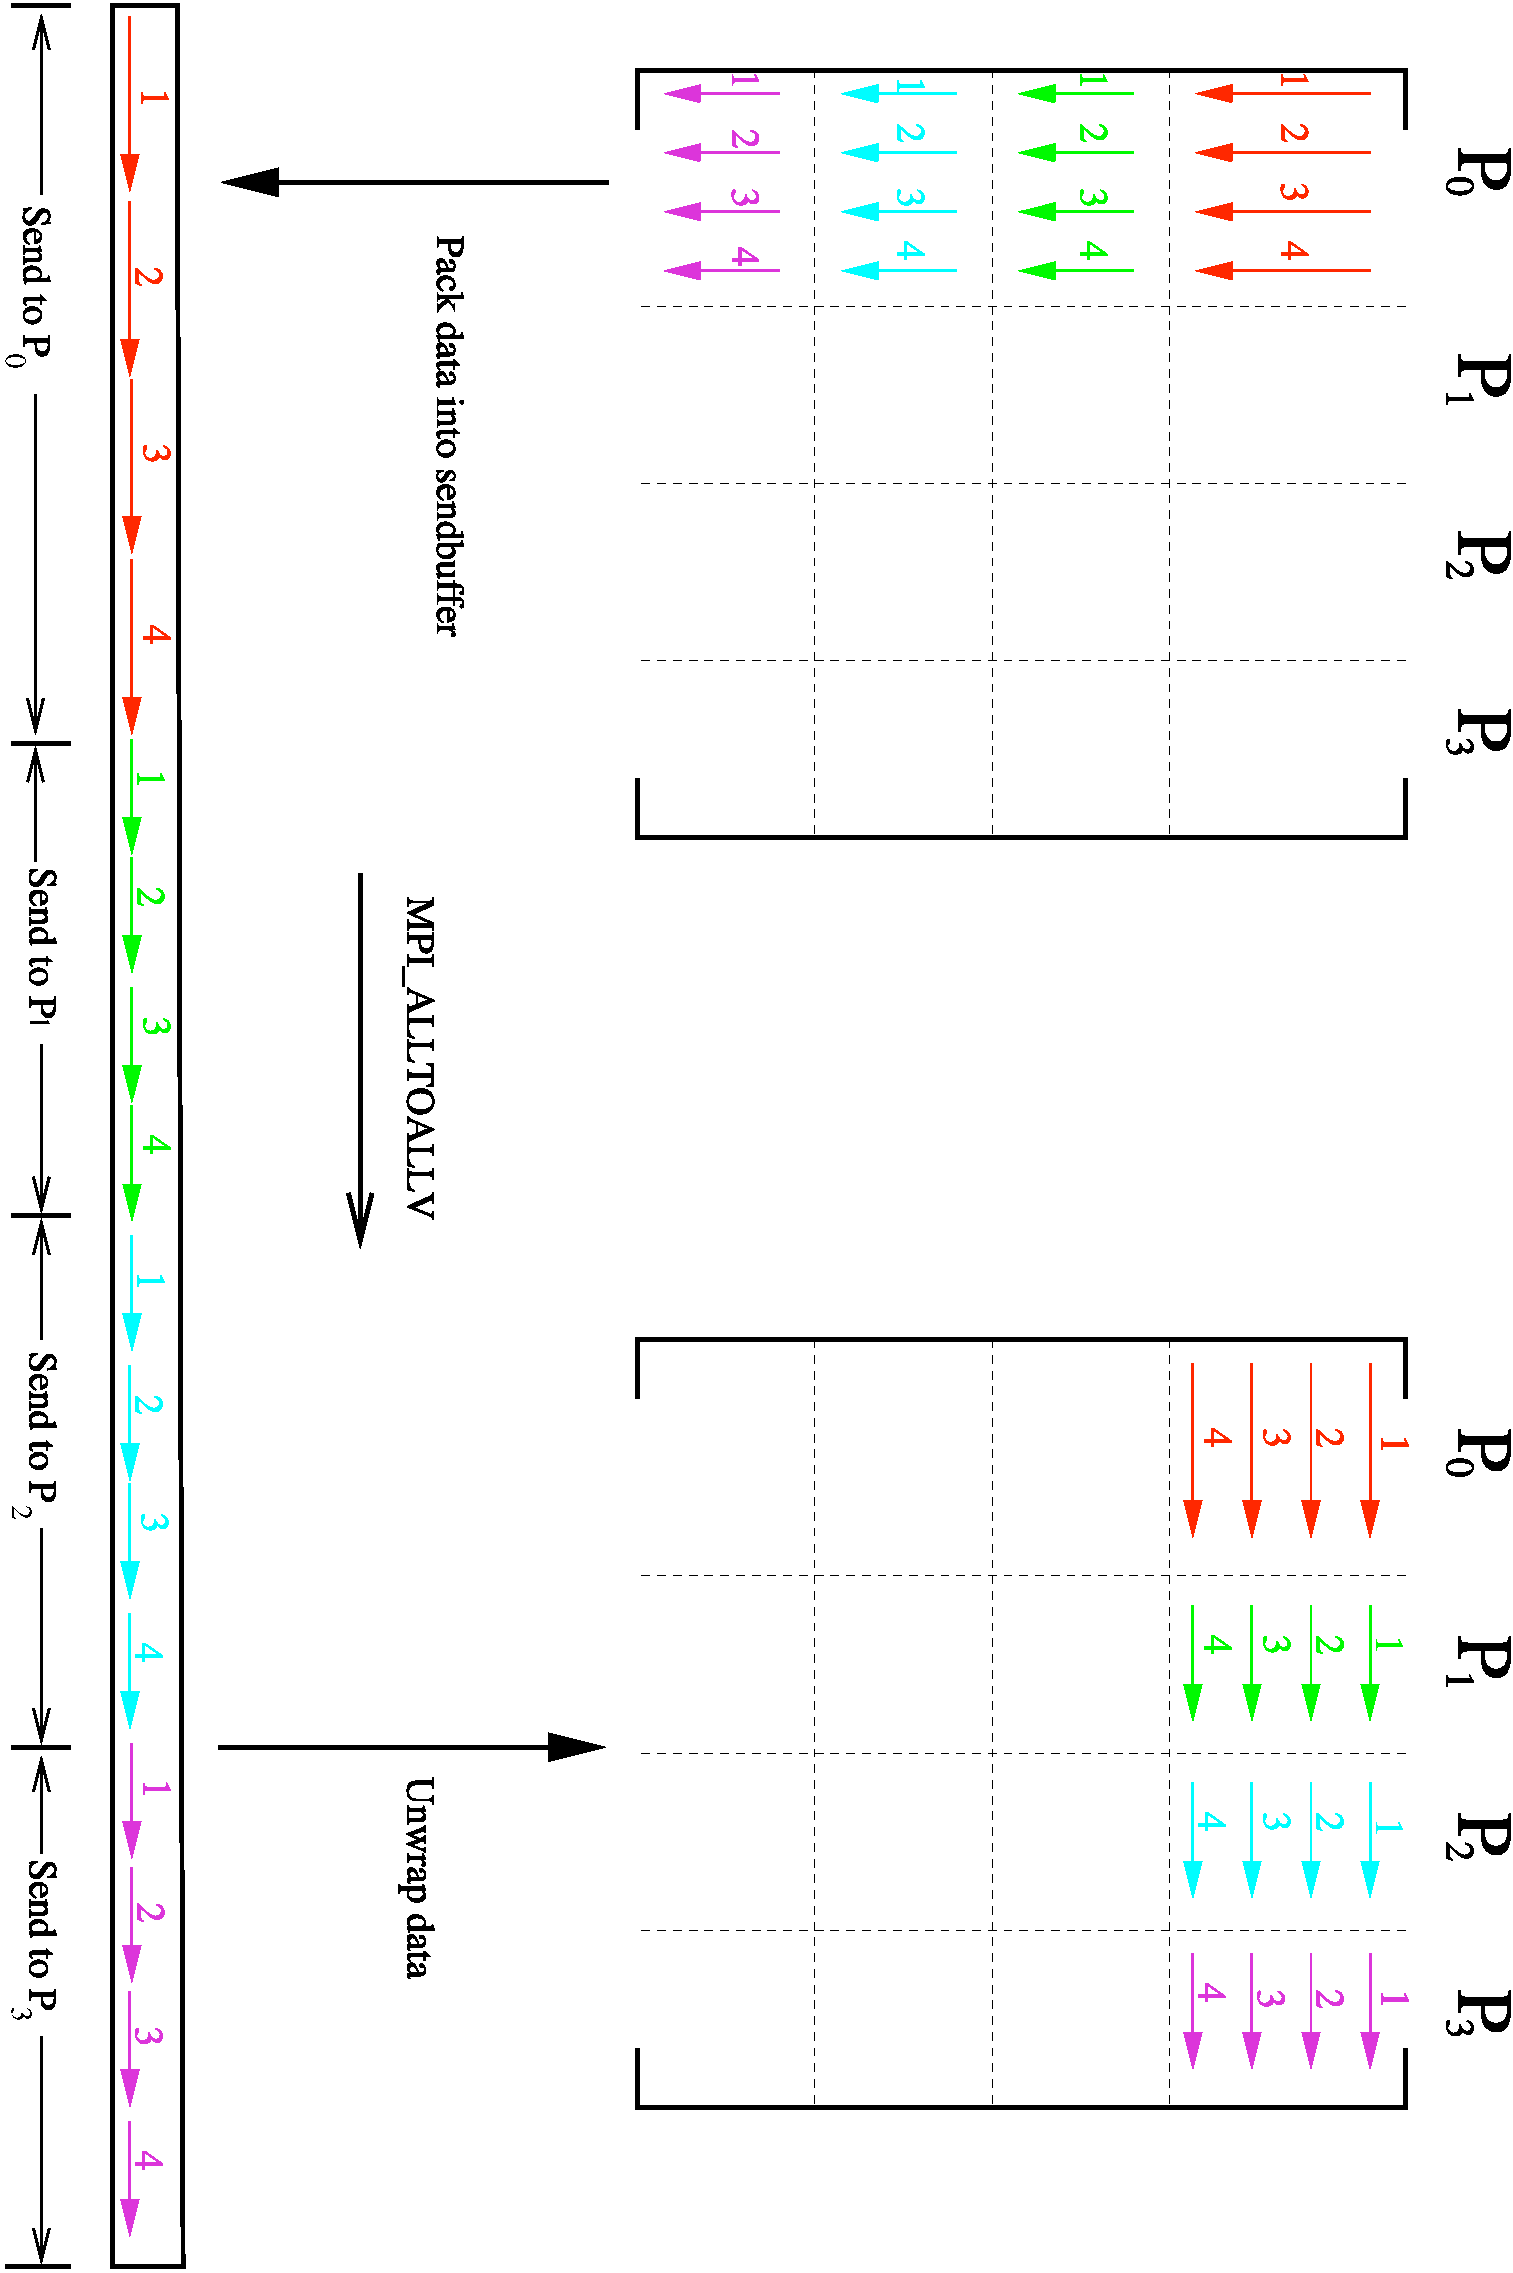
\includegraphics[scale=0.4]{\figs/matrix_blocktranspose}
  \end{center}
  \caption{
    The transpose operation using message passing:
    the packing and unpacking of data.
    The figure is due to Bjarte H{\ae}gland.
  }
  \label{}
\end{figure}

\end{document}
